\chapter{Data processing for OCR}
\label{sec:Data processing for OCR}
The system for character recognition is in similarity to the barcode detection divided in two parts, one for learning and one for testing. However there are some differences in the data processing. The first part of the system consist of the following steps.
\begin{itemize}
	\item Produce training data.
	\item Calculate features.
	\item Use machine learning to train a classifier.
\end{itemize}
The second step consist of the following steps.
\begin{itemize}
	\item Preprocessing of image
	\item Divide the image into tiles of the same size.
	\item Make prediction on each tile with the classifier.
	\item Postprocessing of output
\end{itemize}
Figure \ref{system OCR} illustrates an overview of the system for OCR. Two different classifiers have been used. The first one is trained for separating background from characters and is used with less features than the second classifier. This classifier only has two different classes, false for background and true for characters. The main reason for having this classifier is to make the system faster, hence the features used for this classifier should be as simple and fast as possible.

The second classifier is used to classify individual characters, it is used with an arbitrary number of classes depending on how many different characters that has been used during training.

%Flow chart
\begin{figure}[H]
\centering
\tikzstyle{largeblock} = [rectangle, draw, fill=blue!20, 
    text width=10em, text centered, rounded corners, minimum height=5em]
\tikzstyle{block} = [rectangle, draw, fill=blue!20, 
    text width=6em, text centered, rounded corners, minimum height=4em]
\tikzstyle{line} = [draw, -latex']
\tikzstyle{cloud} = [draw, ellipse,fill=red!20, node distance=3cm,
    minimum height=2em]
 
\begin{tikzpicture}[node distance = 2.5cm, auto]
    % Place nodes
    \node [cloud] (trainingImage) {training data};
    \node [largeblock, below of=trainingImage] (trainingData1) {produce training data and extract features};
    \node [largeblock, below of=trainingData1, node distance=7.5cm] (machine1) {training using Random forest};


     \node [cloud, right of=trainingImage, node distance=4cm] (trainingBack) {training data};
     \node [largeblock, below of=trainingBack] (trainingData2) {produce training data and extract features};
      \node [largeblock, below of=trainingData2] (machine2) {training using Random forest};
     
    \node [cloud, right of=trainingBack, node distance=4cm] (test) {test data};
    \node [block, below of=test] (features1) {extract features};
    \node [block, below of=features1] (classifier1) {Classifier 1};
    \node [block, below of=classifier1] (feature2) {extract features};
    \node [block, below of=feature2] (classifier2) {Classifier 2};
    \node [block, below of=classifier2] (prediction) {prediction};
    
    
    % Draw edges
    \path [line] (trainingImage) -- (trainingData1);
    \path [line] (trainingData1) -- (machine1);
    \path [line] (trainingBack) -- (trainingData2);
     \path [line] (trainingData2) -- (machine2);
    \path [line] (machine2) -- (classifier1);
    \path [line] (machine1) -- (classifier2);
    \path [line] (test) -- (features1);
    \path [line] (features1) -- (classifier1);
    \path [line] (classifier1) -- (feature2);
    \path [line] (feature2) -- (classifier2);
    \path [line] (classifier2) -- (prediction);

\end{tikzpicture}
\caption{Overview of the system for OCR}
\label{system OCR}
\end{figure}

\section{Preprocessing of training dataset}
\label{sec:Preprocessing of training dataset}
The dataset used for training classifiers for character recognition are produced from sample images, one for each character. In this project a special font, OCR-A, has been used. This font has been particularly designed for OCR in a way that makes the character as dissimilar to each other as possible.

\begin{figure}[H]
\centering
	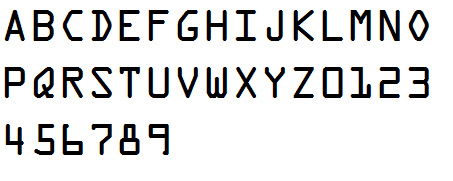
\includegraphics[scale=1]{OCRAfont}
	\caption{Image illustrating OCR A-font}
	\label{Afont}
\end{figure}

From these images a large dataset is produced. This is done by randomly changing the images in different ways depending on what kind of features that will be used later. Every training sample is first resized to the tile size, 54 times 64 pixels. The reason for choosing this size is because all characters are a bit larger in height than in width. An other reason is that the characters normally are written in lines and if the tile is too wide it will enclose more then one character. 

The character is then translated  and rotated randomly  in a way that it still remain mostly inside the tile. Depending what kind of features that are used for the classifier there are some more variations that can be applied to the training samples. Some random noise can be added to the samples. One method during testing is to first threshold the image. In this case it might be a good idea to make some variation of the thickness on the characters for the training data. This can be done by randomly eroding or dilating the sample images. In figure \ref{OCRSample3} two examples of training samples are illustrated for the character 3. The Samples have been translated, rotated and some thinning or thickening have been applied.

\begin{figure}[H]
\centering
	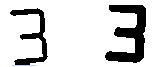
\includegraphics[scale=1]{OCRSample33}
	\caption{Image illustrating two different training samples of the character 3}
	\label{OCRSample3}
\end{figure}

Every character will also be assigned a class label. For example all training samples representing an A will have the class label A. If the characters are written on a line the classifier often make false detections between the characters and also above and under the character. Hence one false class have been added to the training. The training samples for the false class are produced by picking one or two random characters and putting them somewhere at the edge of the tile. In figure \ref{OCRSampleFalse} there is an example of a false sample.

\begin{figure}[H]
\centering
	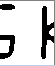
\includegraphics[scale=1]{OCRSampleFalse}
	\caption{Image illustrating an example of a false class}
	\label{OCRSampleFalse}
\end{figure}

\subsection{Character and background separation}
\label{sec:Character and background separation}
The classifier which separates background and characters  is using the same kind of images for training which was described in section \ref{sec:Preprocessing of training dataset} above. In addition random background images are produced and divided into tiles, see figure \ref{randomBackground}.

\begin{figure}[H]
\centering
	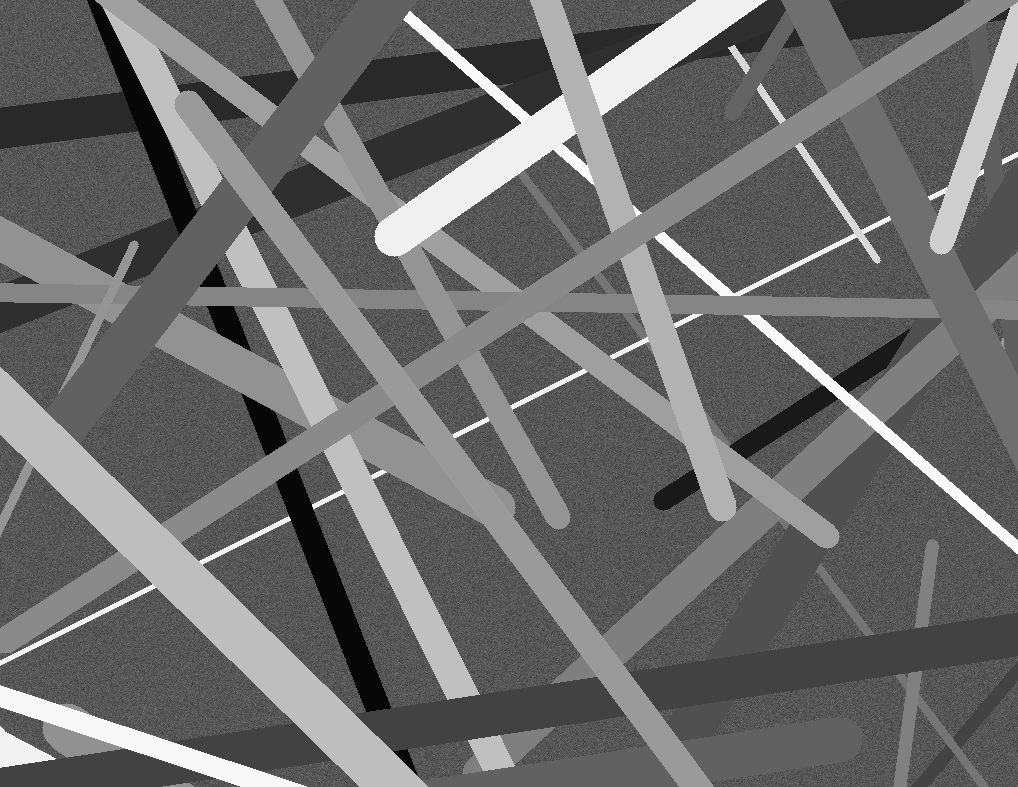
\includegraphics[scale=0.3]{randomBackground}
	\caption{Image illustrating an example of a random background image}
	\label{randomBackground}
\end{figure}

The tiles from the random background images are then labeled as false. The tiles containing characters are labeled as true and tiles containing parts of images illustrated in figure \ref{OCRSampleFalse} are labeled as false.
  
\section{Data processing during testing}
\label{sec:Data processing during testing}
The testing is made on images containing characters of a certain size. The first thing one has to do is to mark one character with a tile so that the height of the tile precisely match the hight of the character, see figure \ref{markTile}.

\begin{figure}[H]
\centering
	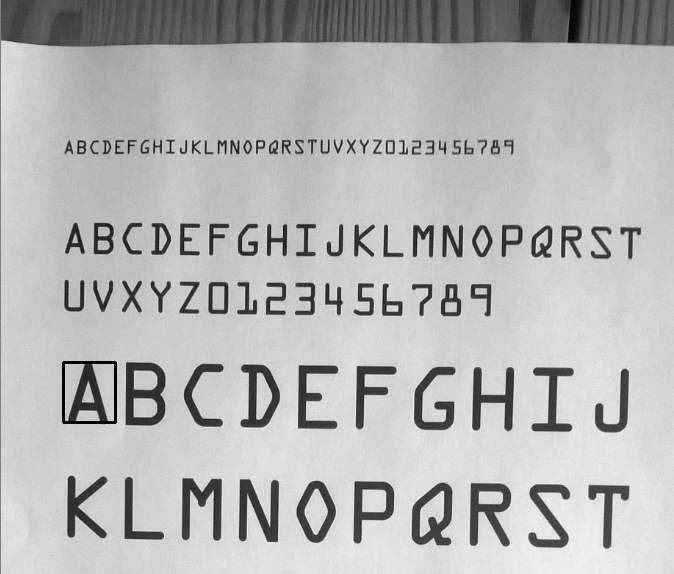
\includegraphics[scale=0.5]{markTile}
	\caption{Image illustrating an test image with a marked character}
	\label{markTile}
\end{figure}

The image will then be resized so that the character which was marked has the same size as the training samples. The image are divided into tiles which can overlap each other and the tiles will be processed one at a time. The system works as illustrated in figure \ref{system OCR}. First features for the first classifier are extracted, then the first classifier is applied. If the amount of trees which classifies the tile as true is above a certain threshold the tile will be passed to the next classifier, otherwise it will be discarded. If the tile is classified as true, new features will be extracted and the second classifier will be applied. If a certain amount of the trees classifies the tile to the same character the tile will get that specific prediction. Figure shows the result from the first classification.

\begin{figure}[H]
\centering
	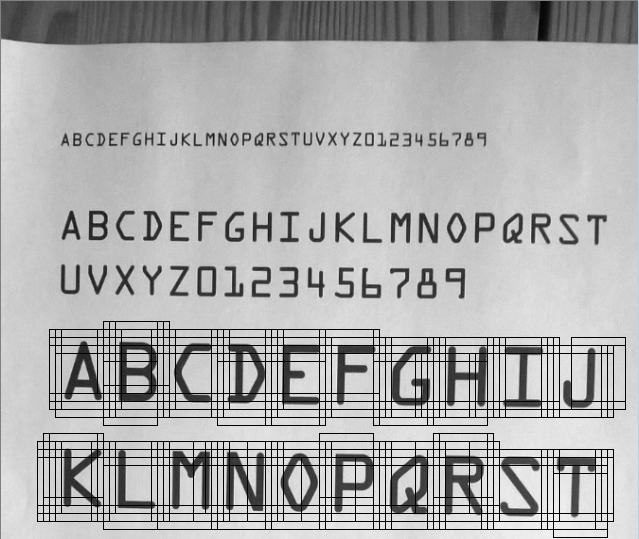
\includegraphics[scale=0.5]{classifier1}
	\caption{Image illustrating the result from the first classification}
	\label{classifier1}
\end{figure}

\subsection{Threshold image}
\label{sec:Threshold image}
One alternative for OCR is to first threshold the images. A good way to do this is to use the adaptive threshold which is implemented in OpenCV. This method divides the image into blocks and thresholds the blocks separately. In each block it calculates the threshold by using a Gaussian window. In figure \ref{thresholdIm} adaptive threshold has been applied to an image.

\begin{figure}[H]
\centering
	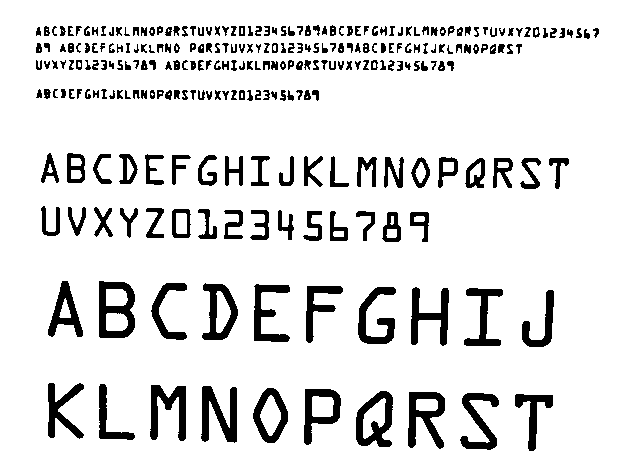
\includegraphics[scale=0.5]{thresholdIm}
	\caption{Image illustrating an image where adaptive threshold has been applied}
	\label{thresholdIm}
\end{figure}

However the classifier can not be the same if it is used directly on the image or if the image is thresholded. If the classifier is trained to be used on the original image the training data needs to have some noise to resemble the test image, this is illustrated in figure \ref{OCRSampleA}.  

\begin{figure}[H]
\centering
	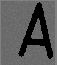
\includegraphics[scale=1]{OCRSampleA}
	\caption{Image illustrating a training sample where some noise has been added}
	\label{OCRSampleA}
\end{figure}
 
If the classifier will be trained to be used on a thresholded image the training data should look as shown in figure \ref{OCRSample3}.

When calculating the point pair features for the two different cases the result will be rather different. For data with noise the features will almost only get the values -1 and 1 since it is rather unlikely that the two points will have the same pixel value. Data which is binary will instead have a lot of features with the value 0 but also features with the values -1 and 1. For that reason it can be assumed that calculating the features on data which is binary will give more information. Both method was tried out and it seemed like the one with binary data worked much better. Since the method to first apply adaptive threshold to the test image also seems to works really good this is the method that has been used further on.
   
\section{Postprocessing}
\label{sec:Postprocessing}
After the classifiers have been applied to the test image a matrix containing all prediction will be received. The matrix will normally contain clusters of predictions. The post processing finds this clusters and calculate the most common prediction in each cluster. Also clusters which are too small can be removed. Since the size of the characters is known it is also possible to remove clusters which are way too big. The amount of prediction in each cluster increases a lot with more overlap. Figure \ref{predictions} illustrates a part of a matrix containing clusters of predictions. 



\begin{figure}[H]
\centering
	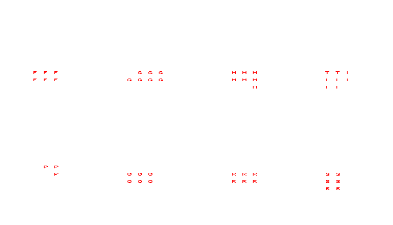
\includegraphics[scale=1]{predictions}
	\caption{Image illustrates a part of the matrix containing clusters of predictions}
	\label{predictions}
\end{figure}
